\chapter{Experimental Setup}

This chapter documents the complete experimental design: hardware and software environment, architectural configurations of the systems under test, workload construction rationale, load scenario definitions, and the precise definitions of all performance metrics reported in Sections 6.1–6.4. Providing this context upfront ensures that numerical results can be correctly interpreted, cross-referenced with the figures, and if necessary independently reproduced by other researchers.

\section{Hardware and Software Environment}

This section describes the technical infrastructure and environmental constraints under which the comparative experiments were conducted. By establishing a strictly controlled, high-performance testing environment, the methodology ensures that all performance metrics—including latency, throughput, and resource consumption—are isolated from external infrastructure noise, thereby providing a consistent baseline for architectural evaluation.

All experiments were executed on a single physical host to eliminate inter-machine network variability between the benchmark client and the systems under test. The benchmark client (k6) ran natively on the host operating system and communicated with containerised services via localhost port bindings, meaning all measured latency is purely attributable to application-layer and container-orchestration processing rather than network infrastructure variability.

\begin{table}[h!]
    \centering
    \caption{System configuration for benchmarking environment}
    \label{tab:system-config}
    \small
    \renewcommand{\arraystretch}{1.2}
    \begin{tabularx}{\textwidth}{l X}
        \toprule
        \textbf{Component} & \textbf{Specification} \\
        \midrule
        CPU & 12th Gen Intel Core i7-12650H — 10 cores (6P + 4E), 2.7 GHz base / 4.7 GHz boost \\
        RAM & 16 GB DDR5 \\
        Operating System & Microsoft Windows 11 Home, Version 10.0.26200 (Build 26200) \\
        Container Runtime & Docker Engine 29.4.1 (build 055a478) \\
        Application Runtime & Node.js v24.11.0 (V8 engine 12.9) \\
        Load Testing Tool & k6 v1.7.1 (commit 9f82e6f1fc, Go 1.26.1, windows/amd64) \\
        Monitoring & \texttt{docker stats} — sampled every 15 seconds via automated PowerShell script \\
        Network Topology & Docker bridge network (benchmark-net); all service endpoints bound to 127.0.0.1 — zero external network hops \\
        \bottomrule
    \end{tabularx}
\end{table}

The decision to adopt a single-host deployment strategy is a strategic choice influenced by the "Experimental Parity" principle found in the research of Al-Debagy and Martinek \cite{Omar_Al-Debagy}. In distributed systems research, external network infrastructure often introduces "jitter"—unpredictable variations in packet delivery—that can obscure the subtle performance differences between architectural styles. By localizing all components on a single Intel Core i7-12650H host, the research focuses exclusively on:.

\section{System-Under-Test: Architecture Configurations}

This section defines the structural configuration of the two architectural candidates subjected to benchmarking. To ensure a scientifically rigorous comparison, the "System-Under-Test" (SUT) is designed around the principle of functional parity, where the internal technical topology is the sole independent variable while the pedagogical business logic remains constant across both environments.

Two functionally identical deployments of the same LMS business logic were benchmarked side by side:

\begin{itemize}
    \item Monolithic: A single NestJS application container (lms\_backend) sharing one PostgreSQL 
    database instance (monolithic-postgres-lms). All inter-module communication occurs via in-process 
    TypeScript function calls within the same Node.js event loop, with no network serialisation or 
    connection pool overhead between modules.
    \item Microservice: Six independent NestJS service containers — AccountService, AcademicService, 
    CourseService, GradingService, Frontend (React/Vite), and Nginx API Gateway — plus a RabbitMQ message 
    broker and per-service PostgreSQL database instances. Inter-service communication uses synchronous 
    REST API calls (routed through Nginx) for latency-critical paths and asynchronous RabbitMQ 
    publish/subscribe messages for eventual-consistency operations such as enrolment confirmations and analytics updates.
\end{itemize}	

Both deployments expose identical REST API endpoints and are seeded with the same database state 
at test start. This functional equivalence ensures that any performance difference is attributable 
to architectural design choices rather than differences in business logic, data volume, or endpoint semantics.

\section{Virtual User Interaction Model}

This section describes the behavioral logic programmed into the benchmarking client to simulate authentic human-system interaction. Unlike static load tests that flood individual endpoints, this model utilizes a stateful execution sequence to replicate a student’s journey through the LMS, ensuring that the performance metrics capture the overhead of session management, database transaction integrity, and inter-service coordination in a realistic operational context.

Each Virtual User (VU) in the benchmark simulates a realistic student session rather than an 
isolated API call. The session consists of four sequential API calls executed in the order below, 
followed by a one-second think time (sleep) before the next cycle begins. This think time prevents 
the test from functioning as a pure throughput flood and instead models the natural pacing of human interaction.

\begin{table}[h!]
    \centering
    \caption{Virtual User Interaction Cycle (4-step sequence, 1 s think time between cycles)}
    \label{tab:user-cycle}
    \small
    \renewcommand{\arraystretch}{1.2}
    \begin{tabularx}{\textwidth}{c l l X}
        \toprule
        \textbf{Step} & \textbf{HTTP Method + Endpoint} & \textbf{Operation Type} & \textbf{LMS Behaviour Simulated} \\
        \midrule
        1 & GET /courses & Read (lightweight) & Browse the course catalogue — most common LMS interaction \\
        2 & GET /courses/:id & Read (moderate) & View full details of a selected course \\
        3 & POST /login & Write (session) & Authenticate user and receive JWT access token \\
        4 & POST /enrollment & Write (DB transaction) & Enrol in the selected course — triggers DB write + RabbitMQ event in Microservice \\
        \bottomrule
    \end{tabularx}
\end{table}

This model is representative of the most common LMS peak-usage scenario: students browsing and enrolling 
in courses at the start of a semester. The mix of read-heavy (Steps 1–2) and write-heavy (Steps 3–4)
 operations within the same VU cycle ensures that both architecture types are exercised under realistic 
 workload heterogeneity, not just pure read or pure write stress.


\section{Load Scenarios}
This section defines the rigorous testing protocols used to stress-test the architectural boundaries of the LMS. By utilizing a diverse range of load patterns—from gradual step increases to instantaneous traffic spikes—the methodology aims to capture the non-linear performance characteristics of both Monolithic and Microservice models, specifically focusing on their resource saturation points and recovery behaviors under extreme operational pressure.

The same VU interaction cycle was applied across the following load scenarios, each designed to stress a 
distinct aspect of architectural behaviour:

\begin{table}[H]
    \centering
    \caption{Load Scenario Definitions}
    \label{tab:load-scenarios}
    \small
    \begin{tblr}{
        colspec = {l l p{3cm} X[j]}, % Điều chỉnh p xuống 3cm để tránh Overfull hbox
        hlines = {0.5pt, gray!50},    % Thay cho \midrule, \bottomrule của booktabs
        vlines = {0.5pt, gray!50},
        row{1} = {font=\bfseries, bg=gray!15},
        stretch = 1.3,               % Sửa lỗi Unknown key rowspread
        cells = {m},                 % Căn giữa nội dung theo chiều dọc
        hline{1,Z} = {1pt},          % Đường kẻ đậm ở đầu và cuối (thay cho \toprule/\bottomrule)
    }
        % Không dùng \toprule ở đây
        Scenario & Pattern & VU Configuration & Architectural Dimension Targeted \\
        % Không dùng \midrule ở đây
        S1 & Step load & 1 $\rightarrow$ 2,000 (12 levels: 1, 5, 10, 15, 20, 50, 100, 200, 500, 1000, 1500, 2000) & Throughput scalability, response-time degradation curve, CPU scaling efficiency \\
        
        S2 & Flash Crowd & All 2,000 VUs injected simultaneously & Peak-load absorption, fail-fast behaviour, event-loop saturation \\
        
        TC1 & CPU Read & Ramp (same 12 levels) - GET /courses & CPU baseline overhead and idle cost of infrastructure processes \\
        
        TC2 & CPU Write & Ramp (same 12 levels) - POST /profile & CPU pressure from DB write transactions and serialisation \\

        TC3 & Mix Load & Ramp (same 12 levels) - POST /profile + GET / courses & CPU pressure from DB write transactions and get transaction \\
        % Không dùng \bottomrule ở đây
    \end{tblr}
\end{table}


Each scenario was executed three times (run1, run2, run3). For CPU timeline visualisation, run1 is 
used as the representative trace (it avoids JVM/Node.js warm-up interference introduced in run2 onward). 
Aggregate metrics — average RPS, average response time, average CPU percentage — are computed across all 
three runs. Any run where host\_total CPU exceeds the mean by more than three standard deviations for 
more than 30\% of the sampling window is flagged as an outlier (typically caused by 
OS-level background process interference) and excluded from aggregate calculations.

\section{Measurement quantities}
This section defines the quantitative metrics and indicators utilized to evaluate the performance and resource efficiency of the systems under test. By establishing precise definitions for throughput, latency percentiles, and computational overhead, the research ensures that the comparative analysis is based on standardized data points, allowing for a transparent identification of the "Performance Tax" and "Resource Contention" inherent in each architectural model.

The following quantity appear throughout measurement process. Each is precisely defined here to prevent ambiguity in interpretation.

\subsection{Throughput (RPS — Requests Per Second)}

The total number of successful HTTP responses (2xx status codes) received by the k6 
client per second, averaged over the steady-state observation window 
at each VU level. This measures the system's processing capacity, 
i.e., how much useful work it can complete per unit time. Higher 
RPS indicates greater system capacity.

In the context of web architectures, this quantity refers to the volume of "useful work" a system can 
process within a specific time window, typically measured in Requests Per Second (RPS). From an architectural 
standpoint, throughput is an indicator of a system's \textbf{Resource Utilization Efficiency}.

\begin{figure}[H]
    \centering/
    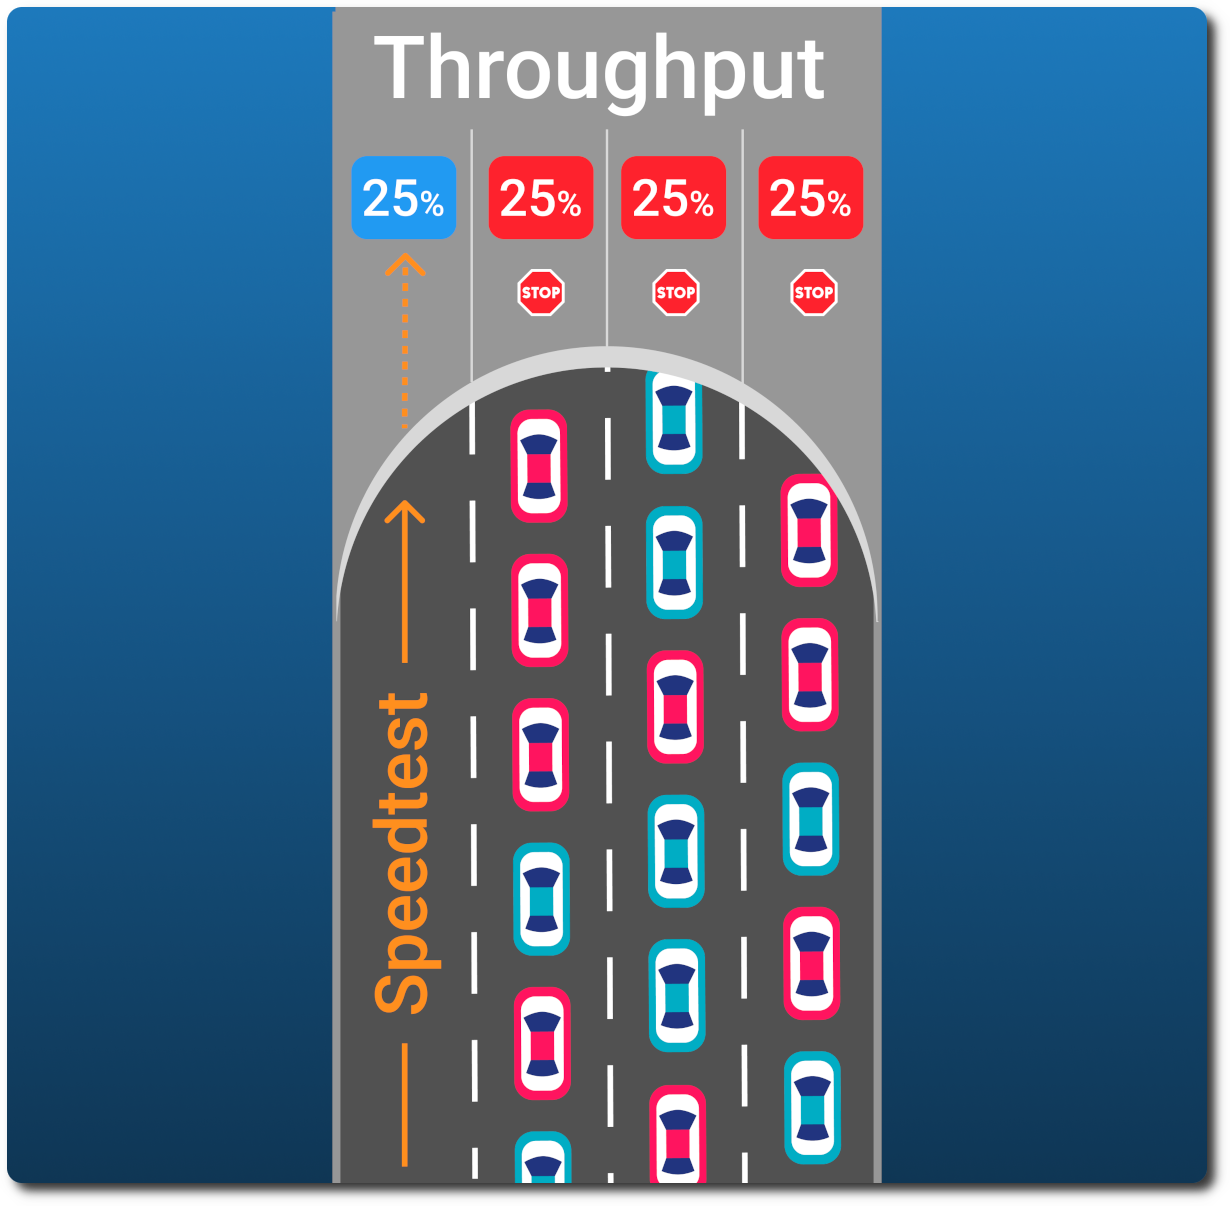
\includegraphics[width=0.65\textwidth]{images/concept/throughput.png}
    \caption{Throughput concept.}
\end{figure}

\subsection{Response Time — Average, P95, and P99}

Response time is the total round-trip latency from when k6 issues an HTTP request to when the full response body 
is received, measured in milliseconds.

\begin{itemize}
    \item Average (mean): The arithmetic mean of all response times within an observation window. The average is sensitive to outliers — a small number of very slow requests can inflate it significantly.
    \item P95 (95th percentile): 95\% of all requests were completed within this time. It characterises the experience of the vast majority of users while filtering out extreme outliers. For LMS deployments, P95 is a stronger indicator of perceived user experience than the mean because it captures the 'typical worst case' a real student would encounter.
    \item P99 (99th percentile): 99\% of all requests were completed within this time. P99 reveals tail-latency behaviour — the performance experienced by the most adversely affected 1\% of users. Under high load, divergence between the average and P99 indicates resource contention or queue starvation (e.g., database connection-pool exhaustion). A P99 value orders of magnitude above the average signals systemic instability rather than random variability
\end{itemize}

Example interpretation: If average = 45 ms, P95 = 210 ms, and P99 = 30,002 ms (as observed for Microservice Write at 200–500 VUs), this indicates that most requests are handled quickly but a small fraction stalls catastrophically — consistent with inter-service coordination timeouts when the request queue exceeds the service's retry budget.



\subsection{CPU Usage and host\_total}

CPU usage is collected via docker stats at 15-second intervals. Docker reports each container's CPU as a percentage of one logical CPU core (100\% = one full core). Therefore, a multi-core system can show container values above 100\% when multiple threads are utilized simultaneously.

\begin{figure}[H]
    \centering/
    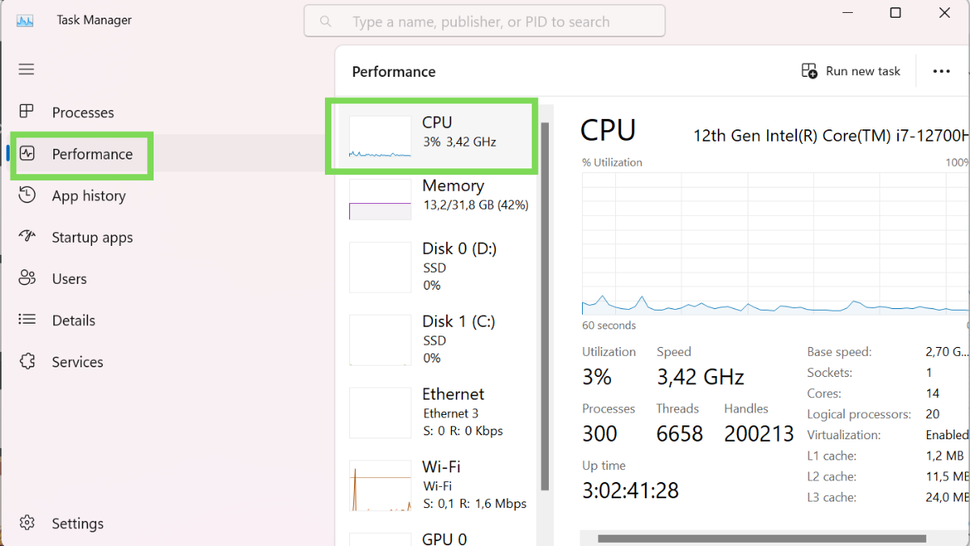
\includegraphics[width=0.65\textwidth]{images/concept/cpu_usage.png}
    \caption{CPU usage concept.}
\end{figure}

host\_total is the sum of all container CPU usages plus the Docker daemon and OS background process overhead. 
This is the single most important metric for fair architecture comparison: it represents the total hardware cost of running the system 
at a given load level, regardless of how that cost is distributed across services. 
Without host\_total, Microservice appears deceptively efficient at the individual-service level while 
concealing the cumulative cost of API Gateway, RabbitMQ, and health-check polling.

\subsection{RAM Usage}

Resident Set Size (RSS) of each container, also collected via docker stats. Reported as the average across the observation window. For the Microservice deployment, the sum of all container RSS values (including message broker and databases) is used.

\begin{figure}[H]
    \centering
    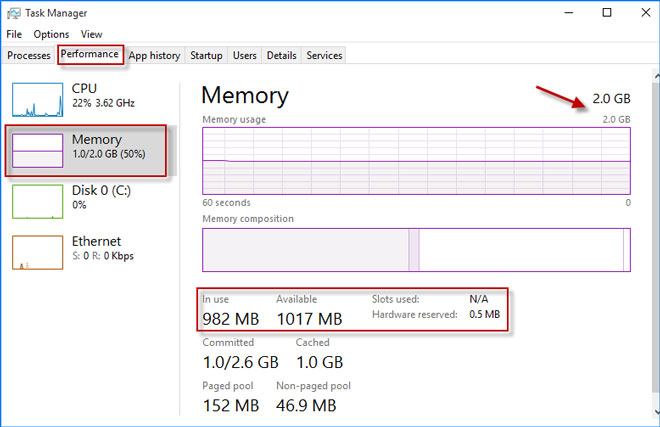
\includegraphics[width=0.65\textwidth]{images/concept/ram_usage.png}
    \caption{RAM Usage Monitoring Concept}
\end{figure}

\section{Metric Definitions}

This section defines the derived metrics which are mentioned in chapter 4 and  used to evaluate the operational efficiency of the architectures beyond raw performance numbers. By introducing the Resource Utilization Efficiency (RUE) framework, the study shifts the focus from "how fast" a system can run to "how much" it costs in terms of computational energy to achieve that speed, providing a quantitative link between software architecture and infrastructure expenditure.

\subsection{Resource Usage Efficiency (RUE)}

As mentioned in section 3.3.4, the Resource Utilization Efficiency (RUE) metric, adopted from Yogant Faye (2025), quantifies how effectively hardware resources are transformed into useful work (processed requests). While the original definition provides a general ratio between workload and provisioned resources, our study adapts and operationalizes this metric to fit the specific context of our empirical experiment.

In this thesis, we define two variants of RUE corresponding to the two primary resources:

\begin{equation}
RUE_{CPU} = \frac{\text{Total Successful Requests}}{\text{Average CPU Usage (\%) during test period}}
\label{eq:rue_cpu}
\end{equation}

\begin{equation}
RUE_{RAM} = \frac{\text{Total Successful Requests}}{\text{Average RAM Usage (MiB) during test period}}
\label{eq:rue_ram}
\end{equation}

where:
\begin{itemize}
    \item \textbf{Total Successful Requests} is the total number of HTTP requests that received a successful response (status code 2xx) during the 5-minute test period, as reported by k6.
    \item \textbf{Average CPU Usage (\%)} and \textbf{Average RAM Usage (MiB)} are the arithmetic means of all resource samples collected throughout the test duration.
\end{itemize}

This formulation differs from the original paper in two important aspects. First, we use \textit{average} resource utilization instead of instantaneous values to account for natural fluctuations in containerized environments. Second, we evaluate RUE across three distinct workload scenarios: \textbf{Idle} (no load), \textbf{Normal load} (200 VUs), and \textbf{Peak load} (1000 VUs).

\subsubsection{Measurement Context}

To ensure a fair and unbiased comparison, each architecture (Monolithic and Microservice) was deployed and measured independently on the same physical host. While one architecture was under test, the other was completely shut down to prevent any resource sharing. For each scenario, the system ran continuously for 5 minutes while a k6 load testing script generated the predefined workload. Resource consumption (CPU and RAM) was monitored every second using Docker Stats and exported to CSV files alongside the number of successful requests.

Before calculating RUE, raw time-series data were aggregated into mean values for the entire test window. This aggregation smooths out short-term spikes and provides a more representative efficiency indicator.

RUE is a particularly valuable metric for cost-efficiency analysis. It normalizes resource consumption by the actual output produced. A system that consumes fewer resources but also processes significantly fewer requests is not necessarily more efficient — its RUE will clearly reveal this limitation. In cloud environments where infrastructure is billed based on CPU-hour or memory-hour, RUE directly correlates with the \textit{cost per successful request}.

The following sections will present the calculated RUE values for both architectures across the three workload scenarios and discuss their implications for cost efficiency.

\subsection{Availability, MTBF, and MTTR}

Our team defines and implements Availability which reflects the \textbf{"Readiness of the Development Environment."} 
Here, the entity that "fails" is not a physical server, but rather the \textbf{workflow} itself. 
Based on completed version of the two architectures, we simulated the entire process of 
making the two architectures from scratch. Our implementation is the strategic use of 
commit logs and Git Log analysis to pinpoint specific milestones and time intervals. The table below is a segment of 
each architect development logs we recorded to mark key milestones.

\begin{figure}[h!]
    \centering
    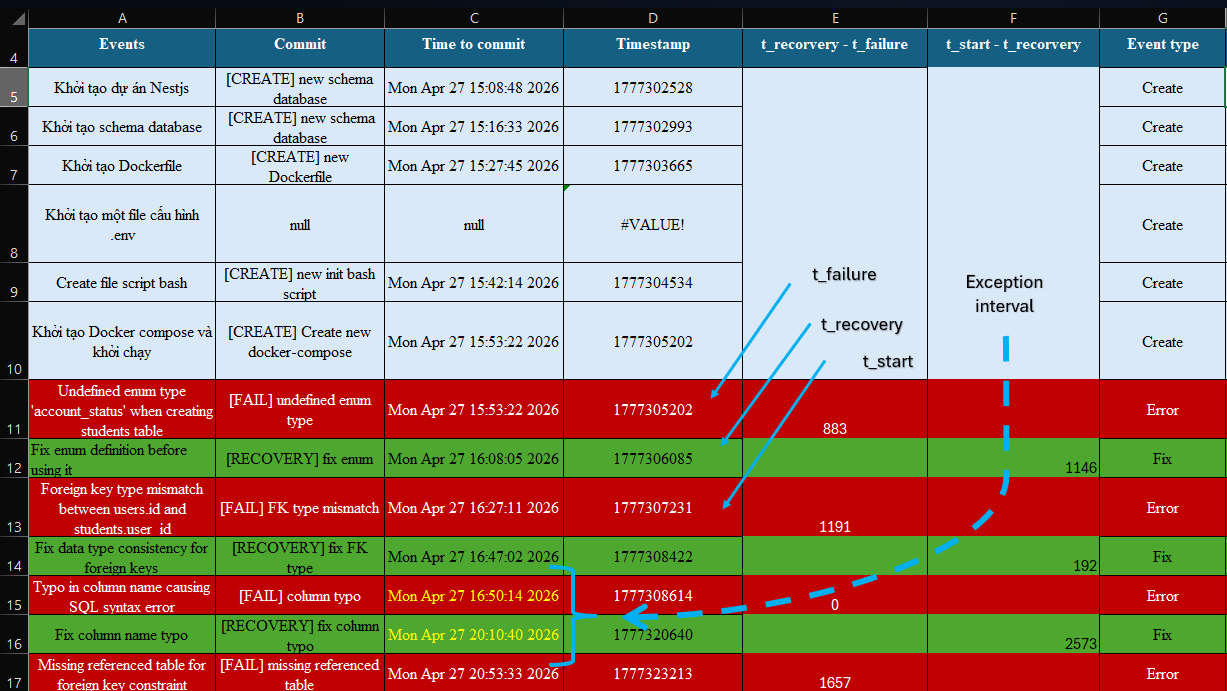
\includegraphics[width=0.8\textwidth]{images/my-demo/tables/Log_commit.png}
    \caption{Example of Log commit history by summary table}
    \label{fig:Log commit history}
\end{figure}

The \textbf{Availability}  metric rely on two components namely \textbf{MTTR} and \textbf{MTBF}. In this context, those are defined as follows:
\begin{itemize}
    \item \textbf{Mean Time Between Failures (MTBF)} is calculated based on the time interval between 
    "Feature Completed" commits, which represent periods where the system is in a stable, functional state.

    \item \textbf{Mean Time To Recovery (MTTR)} is measured as the duration from a commit marking a 
    "Bug Fix" or "Hotfix" until a "Build Success" commit is achieved, signifying the restoration of a ready-to-code environment.
\end{itemize}


This approach allows us to quantify how much of the development time is productive versus how much is lost to 
system-wide or service-specific blockages. By analyzing the sequence of events in the repository, we can 
determine the architectural impact on the development pace.

The systematic recording of these commits requires developers to be constantly present and disciplined 
in their documentation. This rigor is essential to prevent scenarios where exhaustion from long debugging 
sessions leads to forgotten logs or data gaps. 

\subsubsection{Reliability of metrics}

To ensure the validity of \textbf{MTTR} and \textbf{MTBF}, we assume an \textbf{idealized recovery environment}. Our 
team assumes that all developers possess sufficient software development expertise, including proficiency 
in the frameworks and technologies used, as well as strong problem-solving and logical thinking skills. 
This assumption is crucial to isolate the architectural influence, preventing "outlier" data where a simple 
bug might take days to fix due to a developer's lack of foundational knowledge rather than the system's complexity.

However, a practical reality must be acknowledged: in a Monolithic architecture, errors are generally 
easier to locate because there is only a single context to debug, potentially leading to a shorter MTTR
 for individual bugs. Conversely, in Microservice, errors often manifest at the interaction layer between 
 services (e.g., Networking or CORS issues). Even for highly skilled developers, "tracing" an error across 
 multiple distributed services inherently requires more time.

 Furthermore, the disparity in MTTR between the two architectures highlights the trade-off between Local Simplicity and Global Resilience. In a Monolithic system, while the "Cognitive Load" required to trace a bug is low, the "Blast Radius" of a single error is total; a build failure in the Assessment module effectively halts development on the Account module. In contrast, the Microservice architecture, despite having a higher MTTR due to networking complexities, offers Partial Readiness. The higher frequency of FAIL commits in Microservice often reflects its distributed nature where independent components are "tried and tested" in isolation, preventing a localized error from becoming a catastrophic development blockage.

\subsubsection{Handling Data Noise and Outliers}

A significant challenge in measuring development-based availability is the interference 
of external, non-technical factors. Since this experiment aims to measure 
the \textbf{architectural performance} rather than the personal lives of the developers, 
any time intervals that do not contribute to solving technical problems (e.g., rest, personal 
emergencies, or meals) must be identified as "Noise" and excluded from the final calculation.

To maintain the integrity of the temporal data, we establish a threshold 
value, $t_{limit}$. We define the following filtering rules based on the logic of outlier detection:

\begin{equation}
\text{Condition 1: } t^{\text{recovery}}_i - t^{\text{failure}}_i > t^{limit}
\end{equation}
\begin{equation}
\text{Condition 2: } t^{\text{start}}_i - t^{\text{recovery}}_{i-1} > t^{limit}
\end{equation}

If either condition is met, the data point is flagged as an outlier. To illustrate, 
consider a real-world scenario: A developer encounters a database bug at 18:14 and spends 
25 minutes attempting a fix. However, an unexpected personal emergency (e.g., a family accident) 
forces them to abandon the task immediately. The developer returns to work the next morning at 08:04 and completes the fix. 

Without a threshold, the recorded MTTR would inflate to over 13 hours, which is logically absurd 
as it reflects a personal disruption rather than the complexity of the code. By applying $t_{limit}$, 
we classify such intervals as "Invalid." These points are then assigned zero, means that the exception intervals 
are meaningless during system development. This ensures that the resulting Availability percentage 
purely reflects the \textbf{structural characteristics} of Monolithic versus Microservice architectures.

The application of $t_{limit}$ serves as a statistical filter to ensure that the study captures Pure Technical Latency. In software engineering research, "Developer Fatigue" and "External Interruptions" are variables that can skew results toward human performance rather than system design. By enforcing these threshold conditions, the experiment effectively "pauses the clock" during non-productive intervals. This ensures that the calculated Availability ($A$) is a metric of the Architecture’s Friction—the inherent resistance a developer faces when navigating the system’s complexity to resolve a failure.

This methodological pivot from "System Uptime" to "Workflow Readiness" recognizes that in modern DevOps cycles, the primary bottleneck is often not the production stability, but the stability of the incremental delivery pipeline. By quantifying MTBF through the lens of "stable commits," we measure the architecture’s Structural Integrity—its ability to exist in a functional state during active modification. Similarly, MTTR in this context measures Architectural Observability. A high MTTR suggests that the architecture obscures the root cause of failures, forcing developers to spend more time in "investigative stagnation" rather than active coding.

\subsubsection{Simple example}

Take above table \ref{fig:Log commit history} as example. We calculate \textbf{MTTR} and \textbf{MTBF} as follow

\begin{itemize}
    \item \textbf{Mean Time To Recovery (MTTR):} The average duration from $t_{failure}$ to $t_{recovery}$.
    \begin{equation}
    MTTR = \frac{\sum (t_{recovery} - t_{failure})}{n} = \frac{883+1191 + 0 + 1657}{4} = 932.75 \text{ seconds}
    \end{equation}
    \item \textbf{Mean Time Between Failures (MTBF):} The average duration of system uptime (productive development) between failures.
    \begin{equation}
    MTBF = \frac{\sum (t_{failure} - t_{recovery})}{n} = \frac{1146 + 192 + 2573}{3} \approx 1303.66 \text{ seconds}
    \end{equation}
    \item \textbf{System Availability ($A$):}
    \begin{equation}
    A = \frac{MTBF}{MTBF + MTTR} \times 100\% = \frac{1303.66}{1303.66 +  932.75} \times 100\% \approx 58.29\%
    \end{equation}
\end{itemize}

This example shows that there is one interval more than  $7200$, which means that this
performance measurement skips the exception invertal and focusing on continuous time.

Ultimately, the resulting Availability percentage provides a quantitative answer to the "Stability vs. Agility" dilemma. A higher availability in the development environment implies an architecture that supports continuous, uninterrupted workflows. If the data shows that Microservice have a lower MTBF but the ability to maintain independent "up-times" for separate services, it confirms that the architecture is optimized for large-scale, parallel development teams, despite the overhead of distributed debugging. Conversely, a high-availability Monolith would indicate a superior choice for small, rapid-deployment teams where the cost of managing service-to-service communication exceeds the benefits of isolation.

\section{Benchmark Design Rationale}
This section provides the technical and methodological justifications for the specific parameters chosen in the benchmarking suite. By aligning the experimental variables with both the physical constraints of the hardware and the behavioral patterns of real-world academic users, the rationale ensures that the resulting data is not only statistically robust but also contextually relevant to the comparative evaluation of Learning Management Systems.

Several design choices in the benchmark warrant explicit justification:

\begin{description}[style=nextline]
    \item[Why these four API endpoints?] 
    The sequence \texttt{GET /courses} $\rightarrow$ \texttt{GET /courses/:id} $\rightarrow$ \texttt{POST /login} $\rightarrow$ \texttt{POST /enrollment} 
    represents the complete critical path of the most common LMS high-traffic event: a student discovering and enrolling in a course. 
    It combines stateless read operations (Steps 1–2) with stateful write operations involving JWT issuance (Step 3) and a database transaction validated across multiple entities (Step 4). 
    This ensures both architecture types are exercised under the read/write mix characteristic of real peak LMS usage, rather than an artificial uniform-operation benchmark.

    \item[Why 12 VU levels up to 2,000?] 
    Preliminary scoping tests showed that both architectures reached resource saturation (\texttt{host\_total} $>$ 80\%) between 1,000 and 2,000 VUs on the available hardware. 
    The 12-level progression provides sufficient resolution to observe the crossover points at which Microservice' parallel-processing advantage outweighs its coordination overhead, while keeping total benchmark duration manageable.

    \item[Why localhost deployment?] 
    Deploying both systems on a single host eliminates network-layer variability as a confounding factor, allowing observed latency differences to be attributed directly to architectural design (in-process function calls vs. HTTP hops). 
    This design choice is consistent with prior benchmark studies \cite{AlDebagy2018,Schloegl2024} and ensures reproducibility.

    \item[Why three runs per scenario?] 
    A minimum of three runs enables detection of measurement noise caused by OS-level process scheduling, garbage collection pauses in the Node.js V8 engine, and Docker daemon housekeeping. 
    By averaging across runs and applying the outlier-detection threshold described in Section~5.6.2, the reported figures represent stable steady-state behaviour rather than transient artefacts.
\end{description}

These design choices collectively form a rigorous "ceteris paribus" framework, ensuring that the structural topology of the system remains the only significant variable influencing the performance delta. By meticulously isolating infrastructure noise from application logic, the benchmark results presented in the following chapters provide a high-fidelity representation of the architectural trade-offs inherent in modern LMS deployments.